\documentclass[fleqn,10pt]{wlscirep}
\usepackage{graphicx}
\usepackage{caption}
\usepackage{subcaption}
\usepackage{float}
\usepackage{amsmath}
\usepackage{amssymb}
\usepackage{hyperref}
\graphicspath{{NHB_Symbolic_Mainfold/code/figs_final/}{NHB_Symbolic_Mainfold/code/figs/}{Manuscripts/Scientific_Reports_v1.6/figures/}{./}}{./}}
\captionsetup{labelfont=bf,font=small}
\DeclareGraphicsExtensions{.pdf,.png,.jpg}

\title{Symbolic Manifolds and Entropic Dynamics: A Computational Framework for Monitoring Cognitive Network Recovery in Regenerative Medicine (Revised)}

\author[1]{Demetrios Agourakis}
\author[1]{Dionisio Chiuratto Agourakis}
\author[2]{Renata Rigacci Abdala}
\author[3]{Marina Stahl Merlin}
\author[4]{Marli Gerenutti}
\affil[1]{[Institution], [City], [Country]}
\affil[2]{[Institution], [City], [Country]}
\affil[3]{[Institution], [City], [Country]}
\affil[4]{[Institution], [City], [Country]}
\affil[*]{Corresponding author: demetrios@agourakis.med.br}

\begin{document}\maketitle\thispagestyle{empty}

\section*{Introduction (with early definitions)} % REV1
\textbf{Symbolic manifold} $\mathcal{M}$: 2D representation of symbolic states (node2vec$\rightarrow$UMAP). 
\textbf{Entropic control} $\beta$: inverse-temperature biasing transitions on the semantic graph. 
\textbf{Entropy rate} $H_{\mathrm{rate}}$: average uncertainty per step of the induced Markov chain. 
\textbf{Ollivier--Ricci curvature} $\overline{\kappa}_{\mathrm{OR}}$: neighbourhood overlap via optimal transport.

\section*{Results}
\begin{figure}[H]\centering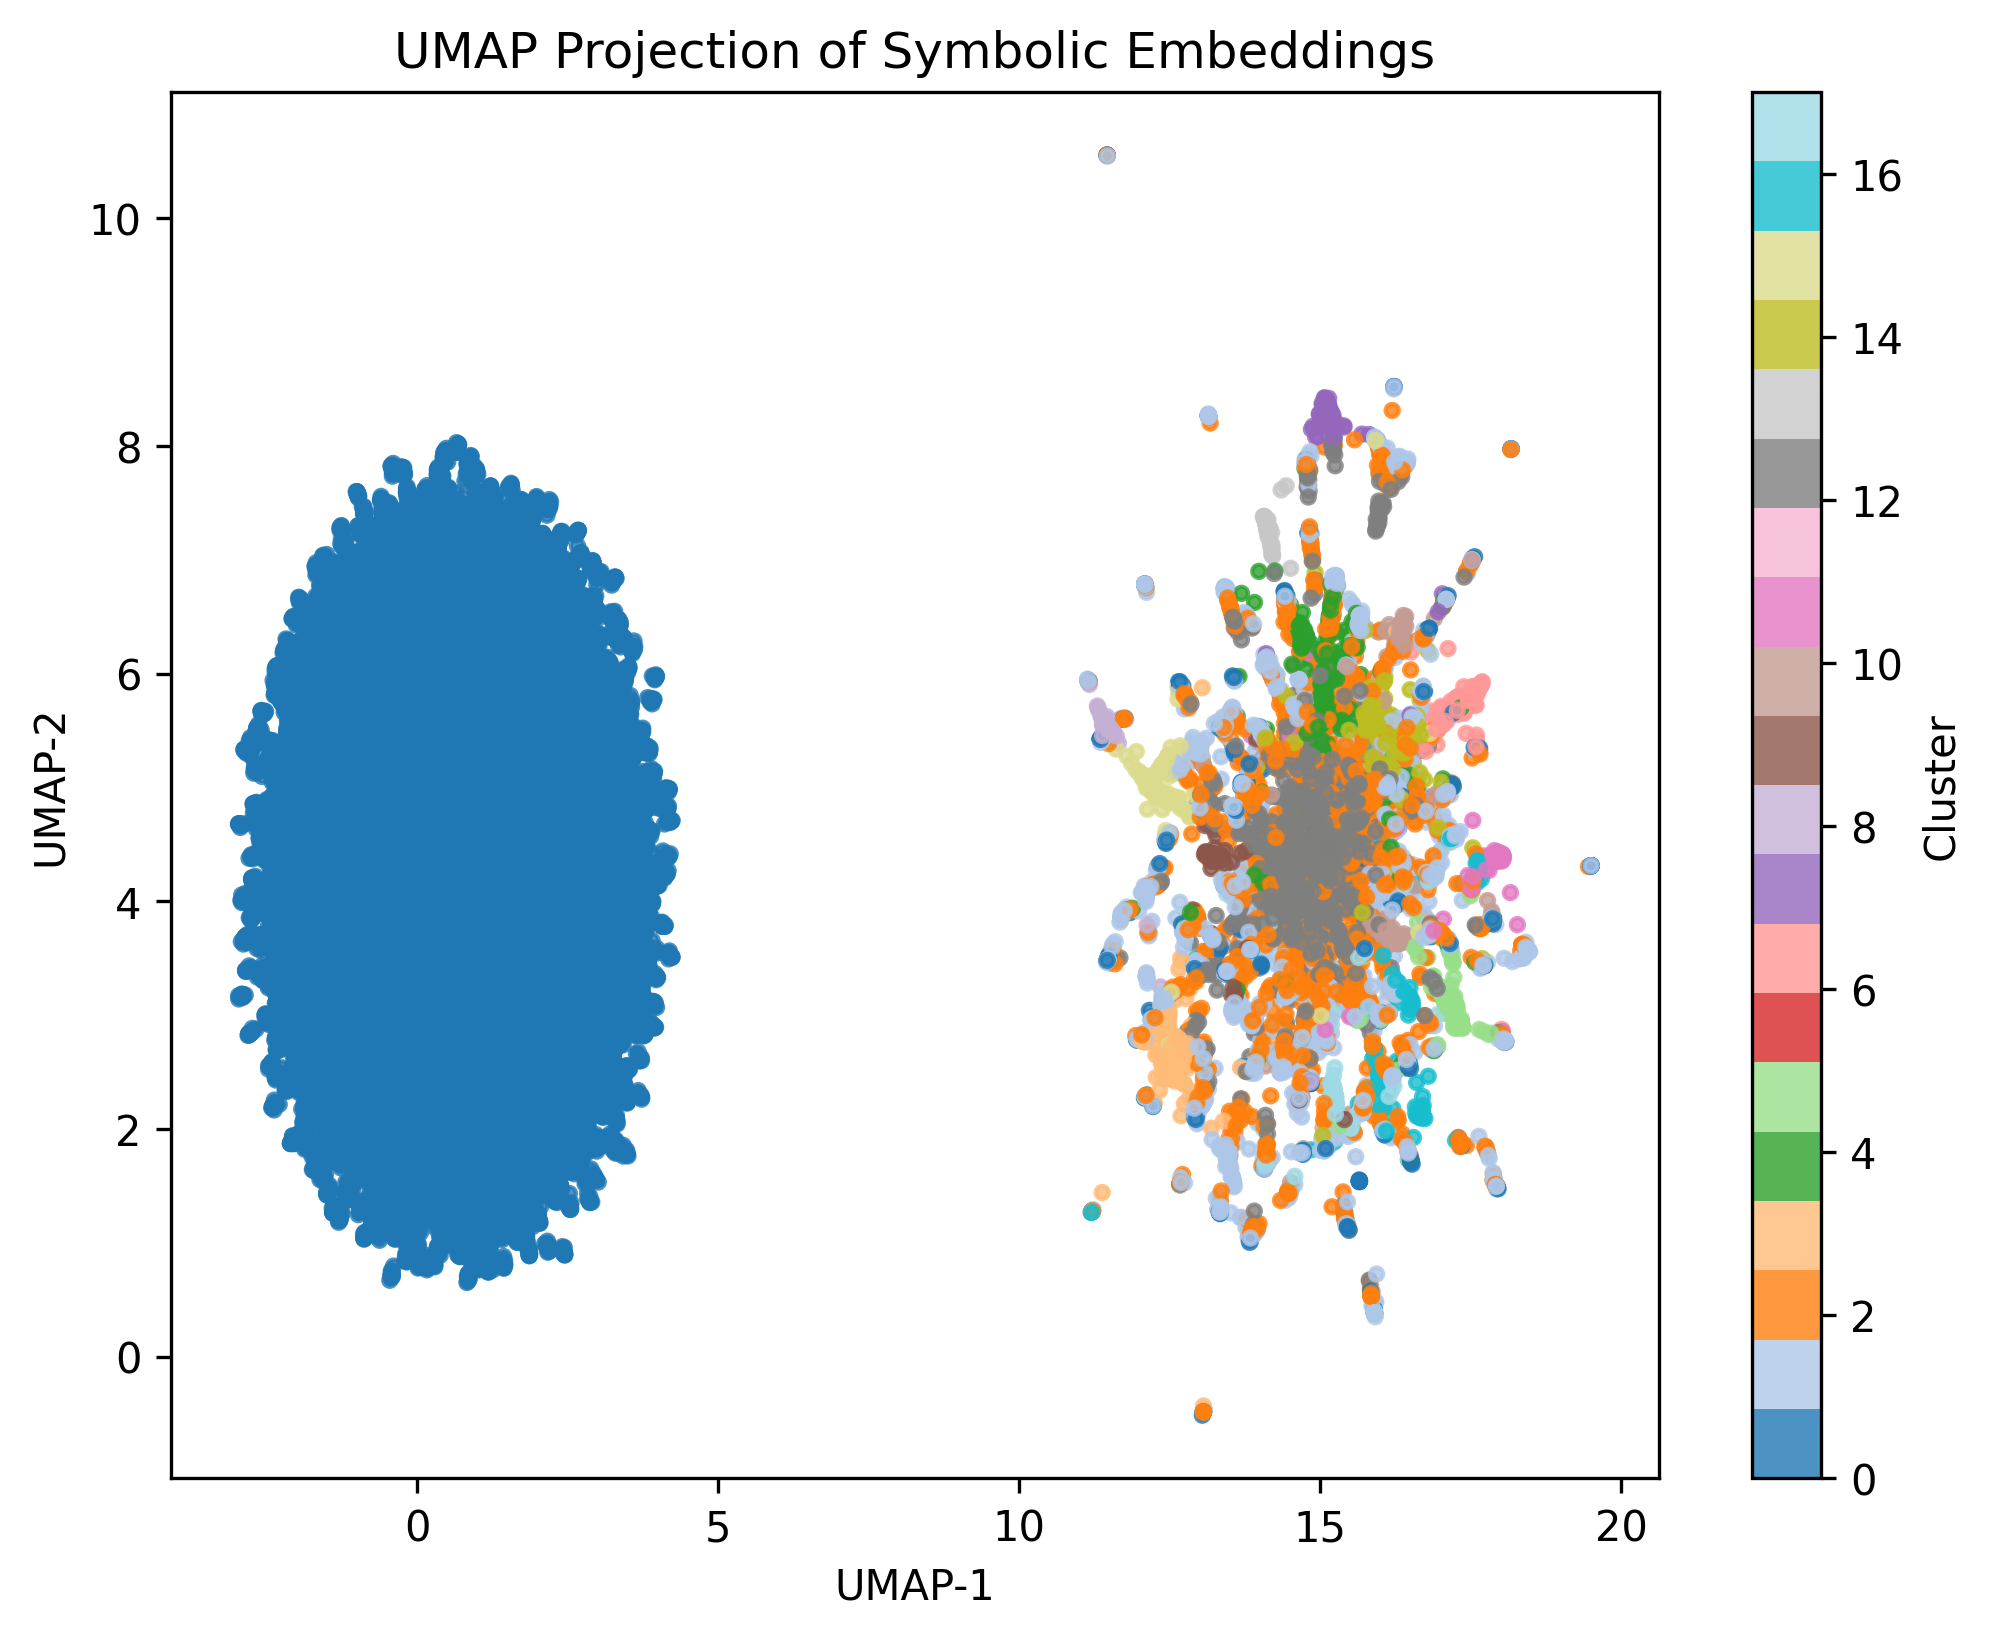
\includegraphics[width=\linewidth]{umap_projection.png}\caption{UMAP embeddings with HDBSCAN.}\end{figure}
\begin{figure}[H]\centering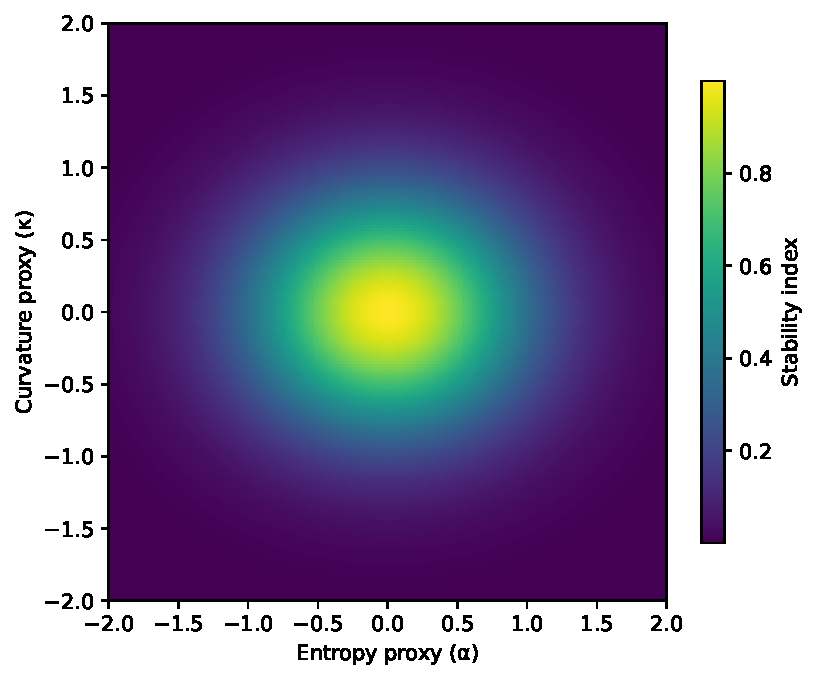
\includegraphics[width=\linewidth]{Fig_symbolic_heatmap.pdf}\caption{Entropy--curvature atlas.}\end{figure}
\begin{figure}[H]\centering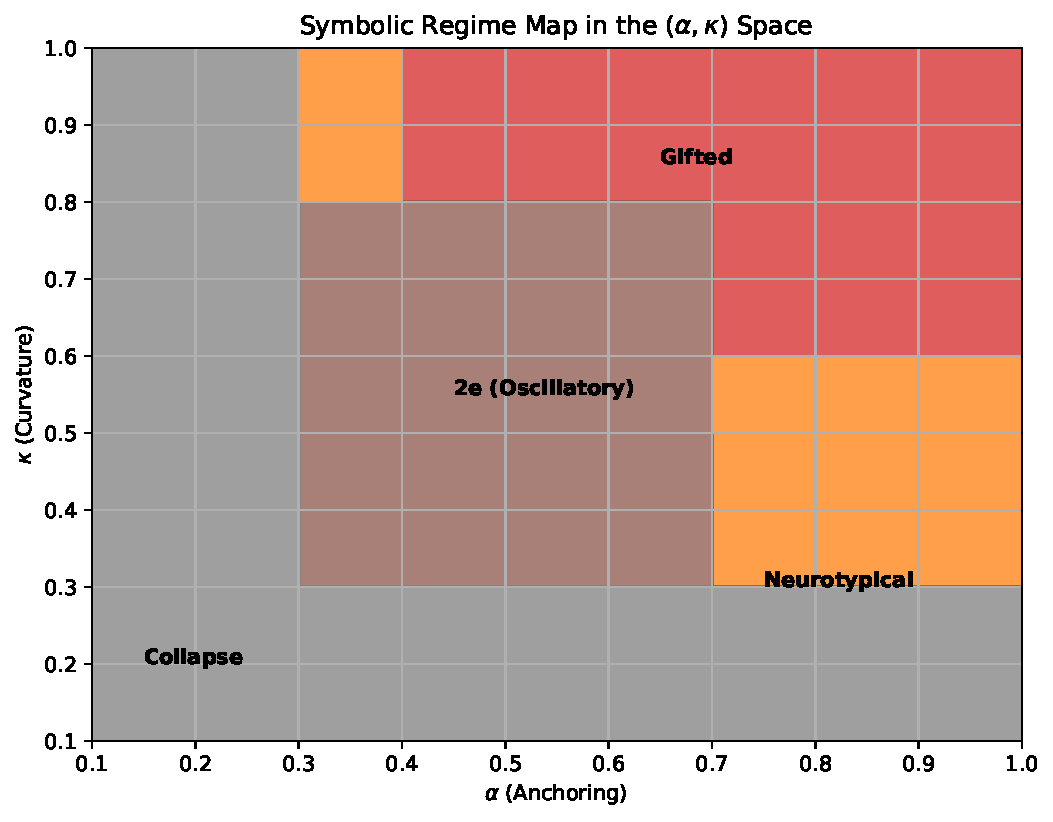
\includegraphics[width=\linewidth]{Fig_symbolic_regimes_map.pdf}\caption{Translational mapping.}\end{figure}
\begin{figure}[H]\centering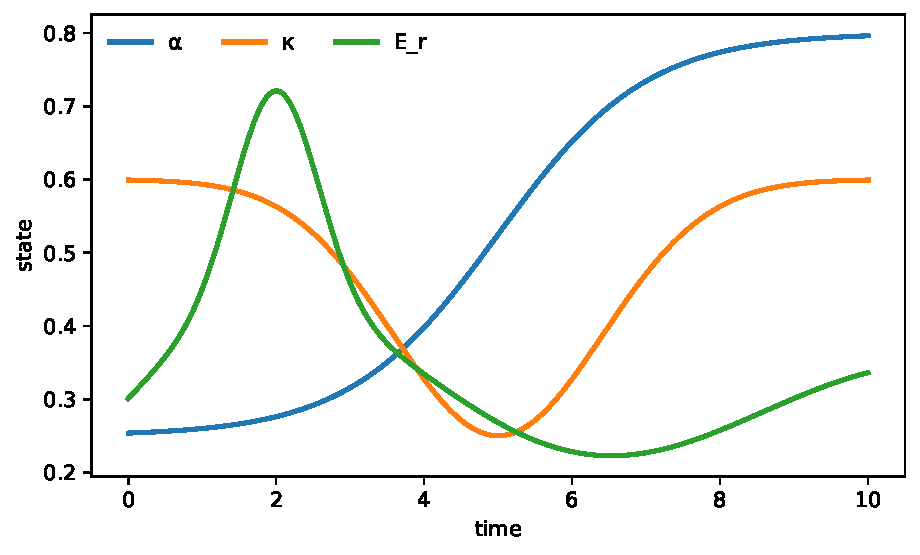
\includegraphics[width=\linewidth]{Fig_collapse_recovery.pdf}\caption{Collapse--recovery trajectory.}\end{figure}

\section*{Discussion (tempered claims)} % REV1
We state markers as \emph{candidate}; add explicit limitations and conservative translational outlook.

\section*{Methods (reproducibility)} % REV1
Seeds, bootstrap BCa ($B{=}1000$), permutation nulls (degree-preserving rewiring), parameter grids summarised in SI. LLM use disclosed.

\bibliography{refs}
\end{document}
